\documentclass[12pt, a4paper]{article}

\usepackage[czech]{babel}
%\usepackage[IL2]{fontenc}
\usepackage[utf8]{inputenc}
\usepackage{enumitem}
\usepackage{parskip}
\usepackage{tocloft}
\usepackage{multicol}
\usepackage[hidelinks]{hyperref}
\usepackage{graphicx}
\usepackage{float}
\usepackage{listings}
\usepackage{xcolor}
\usepackage{amsmath}
\usepackage{tikz}

% Define code style for C
% Define code style for C with proper handling of Czech characters
\lstset{
    language=C,
    basicstyle=\ttfamily\small, % Přidání \small pro lepší čitelnost
    keywordstyle=\color{blue},
    stringstyle=\color{red},
    commentstyle=\color{gray},
    breaklines=true,
    frame=shadowbox,
    numbers=left,
    numberstyle=\tiny\color{gray},
    stepnumber=1,
    numbersep=5pt,
    showstringspaces=false,
    tabsize=4,
    captionpos=b,
    literate=
        {á}{{\'a}}1
        {č}{{\v{c}}}1
        {ď}{{\v{d}}}1
        {é}{{\'e}}1
        {ě}{{\v{e}}}1
        {í}{{\'i}}1
        {ň}{{\v{n}}}1
        {ó}{{\'o}}1
        {ř}{{\v{r}}}1
        {š}{{\v{s}}}1
        {ť}{{\v{t}}}1
        {ú}{{\'u}}1
        {ů}{{\r{u}}}1
        {ý}{{\'y}}1
        {ž}{{\v{z}}}1
        {Á}{{\'A}}1
        {Č}{{\v{C}}}1
        {Ď}{{\v{D}}}1
        {É}{{\'E}}1
        {Ě}{{\v{E}}}1
        {Í}{{\'I}}1
        {Ň}{{\v{N}}}1
        {Ó}{{\'O}}1
        {Ř}{{\v{R}}}1
        {Š}{{\v{S}}}1
        {Ť}{{\v{T}}}1
        {Ú}{{\'U}}1
        {Ů}{{\r{U}}}1
        {Ý}{{\'Y}}1
        {Ž}{{\v{Z}}}1
}



\begin{document}

%Uvodni strana
\begin{titlepage}
    
\includegraphics[width=0.75\textwidth]{img/fav.png}
    \begin{center}


        \vspace{2cm}

        \Huge
        Semestrální práce KIV/UPS

        \vspace{1cm}

        \LARGE
        Úvod do počítačových sítí

        \vfill

        \vspace{0.5cm}

        \normalsize
        \raggedright
        Student:        Adam Míka \\
        Osobní číslo:   A22B0319P \\
        Email:          mikaa@students.zcu.cz \\
        Datum:          22. ledna 2025
        \vspace{0.2cm}

    \end{center}
\end{titlepage}

%tečky v obsahu
\renewcommand{\cftsecleader}{\cftdotfill{\cftdotsep}}
\renewcommand{\cftsubsecleader}{\cftdotfill{\cftdotsep}}
\renewcommand{\cftsubsubsecleader}{\cftdotfill{\cftdotsep}}

%obsah
\setcounter{page}{2}
\tableofcontents
\listoffigures
\lstlistoflistings
\begin{thebibliography}{99}
  \end{thebibliography}
\pagebreak


\section{Zadání}
\large
\textbf{Hlavní cíle:}
\normalsize
Zbytek zadání zde: \href{https://home.zcu.cz/~ublm/files/PozadavkyUPS.pdf}{\textcolor[RGB]{20,20,200}{\underline{\textit{PDF}}}}


\section{Analýza úlohy}

Základem této práce je zrealizovat síťovou hru „Rock-Paper-Scissors“ (kámen, nůžky, papír) mezi dvěma hráči, kteří společně odehrají několik kol (typicky 10). Aplikace se skládá z~\textbf{TCP serveru} a~\textbf{klientské aplikace}, přičemž mezi nimi probíhá výměna dat podle jednoduchého vlastního protokolu.

Z hlediska analýzy byly zjištěny následující klíčové požadavky:
\begin{itemize}
    \item \textbf{Stavová logika a sledování průběhu hry:} Každý hráč může být v~různých stavech (např. \texttt{LOBBY}, \texttt{PLAYING}, \texttt{RECONNECTING}), přičemž přechod do jiného stavu je řízen příchozími zprávami (\texttt{login}, \texttt{ready}, \texttt{game}, \ldots).
    \item \textbf{Definovaný formát zpráv:} Veškerá komunikace používá formát s~prefixem \verb|RPS| a~jednotlivé části zprávy jsou odděleny znakem \texttt{|}. Zprávu ukončuje středník (\texttt{;}).
    \item \textbf{Jednoduchá kontrola validity:} Server i klient kontrolují, zda je prefix \verb|RPS| přítomen, zda následuje očekávaný typ zprávy (např. \texttt{login}, \texttt{ping}, \texttt{game}) a zda je dle herního stavu tato zpráva povolena. Nevalidní zpráva se okamžitě odmítá.
    \item \textbf{Přesné řízení průběhu herního kola:} Hráči nezávisle odešlou své volby (\emph{rock}, \emph{paper}, \emph{scissors}), server vyhodnotí výsledek a~aktualizuje skóre (v rámci \texttt{score|x|y;} zprávy).
    \item \textbf{Obsluha odpojení a reconnect:} Aplikace řeší situace, kdy jeden z hráčů ztratí spojení. Server hráče dočasně označí jako \texttt{RECONNECTING} a~pokud se připojí zpět, hra může pokračovat. V~případě trvalého odpojení je druhý hráč přesunut zpět do \texttt{LOBBY}.
\end{itemize}

Součástí implementace je také mechanismus \texttt{ping--pong}, který slouží ke zjištění dostupnosti klienta, popř. k~detekci neaktivních klientů v~důsledku chyb na síti. Celkově tak aplikace zajišťuje robustnost a konzistenci probíhajícího zápasu. Výsledkem je funkční a přehledné řešení pro multiplayerovou hru s~možností obsluhy více hráčů a~jednoduchou správou hry na úrovni serveru.


\section{Popis síťového protokolu}

\subsection{Základní formát zprávy}
Každá zpráva mezi klientem a~serverem začíná tzv. \textit{magickým prefixem} \verb|RPS| a~má strukturu:
\[
  \text{RPS}|\,\langle\text{příkaz}\rangle\,|\,\langle\text{data}\rangle;
\]
Znak \texttt{;} ukončuje jednu logickou zprávu.

\subsection{Typy zpráv}

V této sekci jsou uvedeny typy zpráv používané v komunikačním protokolu aplikace Rock-Paper-Scissors. Zprávy jsou rozděleny na dvě kategorie: \textbf{zprávy odesílané z klienta na server} a \textbf{zprávy odesílané ze serveru na klienta}.

\subsubsection{Příklady zpráv z klienta na server}
\begin{itemize}
  \item \texttt{RPS|login|Alice} -- Klient žádá o přihlášení se jménem \uv{Alice}.
  \item \texttt{RPS|ping} -- Klient zasílá dotaz typu \emph{heartbeat}.
  \item \texttt{RPS|ready|Alice} -- Klient se hlásí jako připraven zahájit hru.
  \item \texttt{RPS|game|rock} -- Klient posílá svou volbu \uv{kámen}.
  \item \texttt{RPS|reconnect|Alice} -- Pokud dojde k odpojení klienta, při opětovném připojení klient posílá tuto zprávu na server.
  \item \texttt{RPS|return\_to\_lobby} -- Po ukončení hry klient posílá zprávu na server jako informaci o připojení do lobby pro další hru.
  \item \texttt{RPS|delete} -- V případě vypnutí klienta kliknutím na křížek klient posílá tuto zprávu na server.
\end{itemize}

\subsubsection{Příklady zpráv ze serveru na klienta}
\begin{itemize}
  \item \texttt{RPS|connected;} -- Server potvrzuje, že uživatel \uv{Alice} se úspěšně přihlásil.
  \item \texttt{RPS|pong;} -- Server odpovídá na \emph{ping} zprávu.
  \item \texttt{RPS|Group 1|opponent\_name;} -- Server oznamuje klientovi, že byl zařazen do skupiny \texttt{Group 1} s protivníkem \texttt{opponent\_name}.
  \item \texttt{RPS|start;} -- Server oznamuje začátek hry.
  \item \texttt{RPS|score|1|2;} -- Server posílá aktuální stav skóre (\texttt{player\_score = 1}, \texttt{opponent\_score = 2}).
  \item \texttt{RPS|opponent\_disconnected;} -- Pokud dojde k dočasnému odpojení klienta, server posílá zprávu, aby klient počkal na opětovné připojení protivníka.
  \item \texttt{RPS|opponent\_reconnected;} -- Oznámení, že se klient znovu připojil a hra může pokračovat.
  \item \texttt{RPS|return\_to\_waiting;} -- Pokud vyprší čas na připojení, server informuje klienta, aby se přesunul zpět do lobby pro další hru.
  \item \texttt{RPS|error|Invalid action;} -- Server vrací chybový stav klientovi, pokud klient provedl neplatný tah nebo jinou chybu.
\end{itemize}

\begin{figure}[h!]
    \centering
    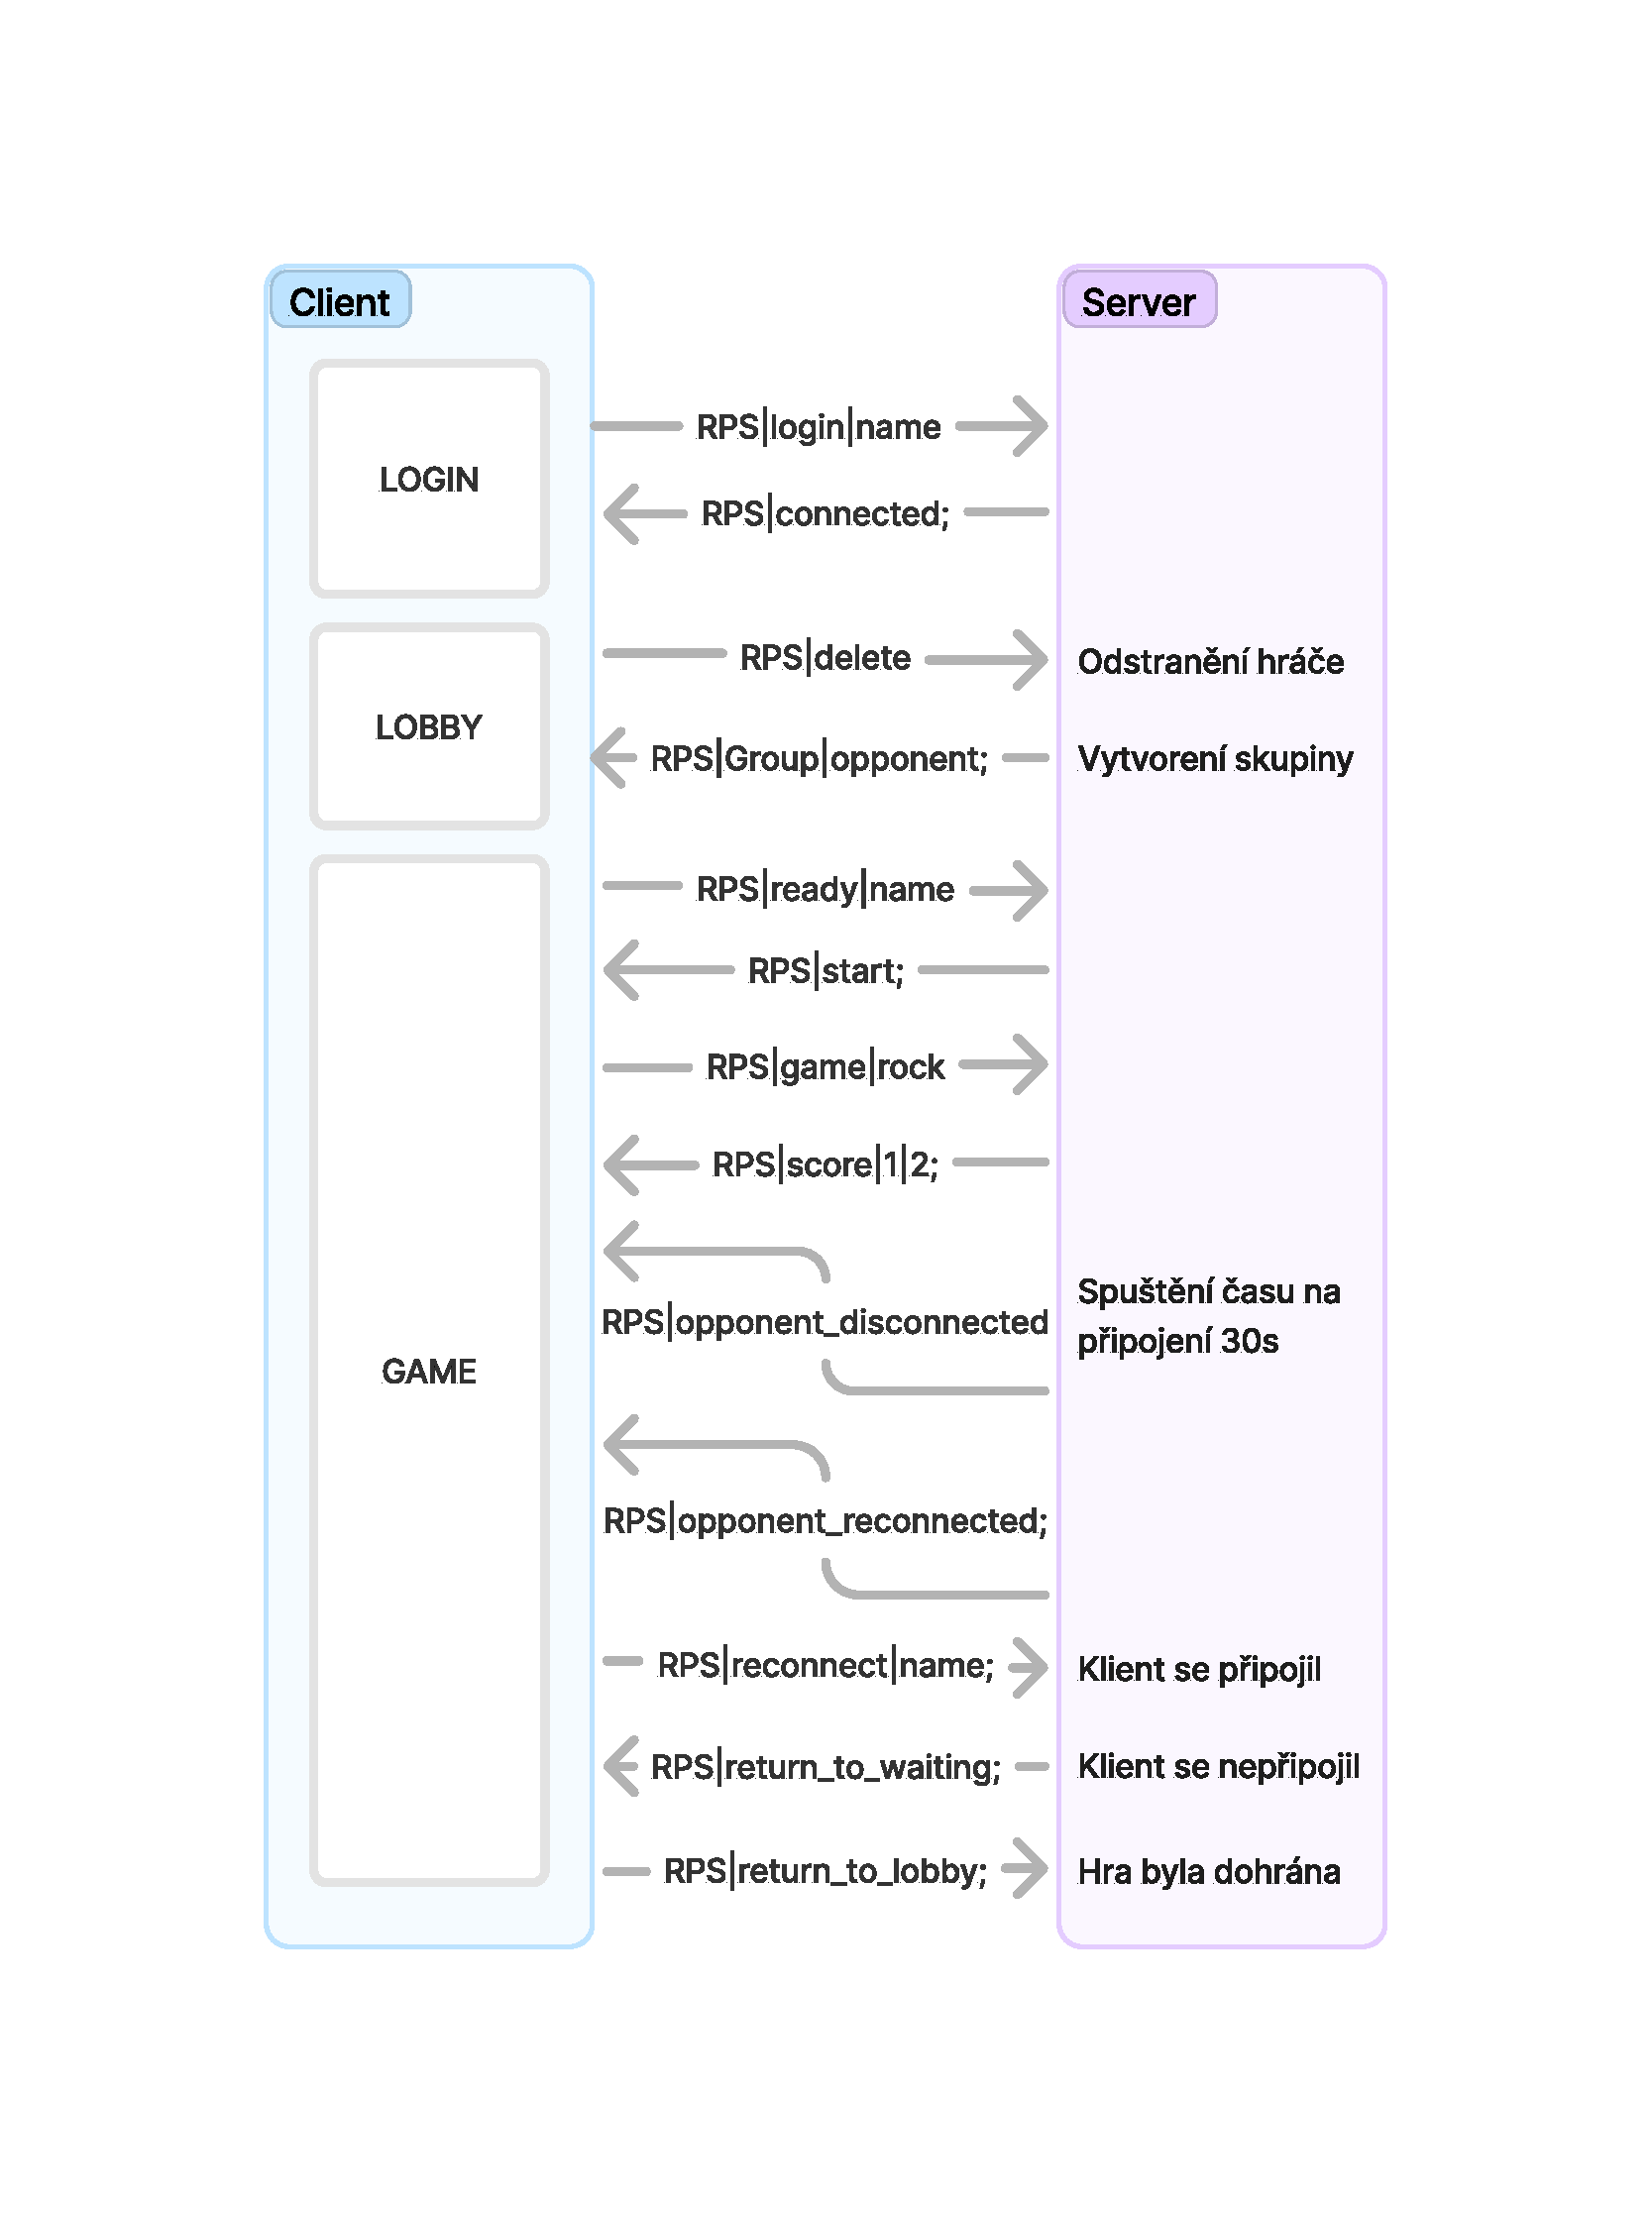
\includegraphics[width=\textwidth]{img/diagram.pdf} % Cesta k PDF souboru
    \caption{Diagram komunikace serveru a klienta}
    \label{fig:diagram}
\end{figure}

\newpage
\subsection{Validace zpráv}
Validace zpráv v tomto programu se provádí kontrolou formátu, obsahu a také kontrolou souvislosti se stavem hráče. Zpráva je vždy rozdělena rourou (``|``) na několik částí, z nichž první bývá prefix (například ``RPS``) identifikující protokol, a další části nesou informaci o typu zprávy (jako ``login``, ``ready``, ``game``) a konkrétních datech (např. ID hráče nebo volba ``rock/paper/scissors``). Pokud je formát neúplný, neodpovídá očekávanému prefixu nebo pokud zpráva nedává smysl z hlediska herního stavu hráče, je vyhodnocena jako nevalidní.

\paragraph{Typické příklady chybně formátovaných nebo nevalidních zpráv:}
\begin{enumerate}
    \item \texttt{ABCD|login|muj-hrac}
    \textit{- Prefix ``ABCD`` je neplatný (chybí ``RPS``).}

    \item \texttt{RPS|ping} od hráče, který ještě neprošel \texttt{login}
    \textit{- Server nezná ID daného hráče (stav ``Unknown player``), proto je zpráva vyhodnocena jako nevalidní.}

    \item \texttt{RPSloginmuj-hrac}
    \textit{- Chybějí oddělovače ``|`` i prefix ``RPS``. Je to jeden nepravidelný řetězec.}

    \item \texttt{RPS||ready}
    \textit{- Za prefixem ``RPS`` chybí typ zprávy. Volná roura navíc signalizuje chybějící část.}

    \item \texttt{RPS|game|scissors} od hráče, který ještě není ve stavu \texttt{PLAYING}
    \textit{- Hráč musí být nejprve \texttt{login}, poté \texttt{ready}, aby mohl posílat herní tah. Server proto zprávu odmítne.}

    \item \texttt{RPS|ready|}
    \textit{- Za slovem \texttt{ready} chybí ID hráče. Není možné ověřit, kdo tuto zprávu posílá.}

    \item \texttt{RPS|error|XYZ}
    \textit{- Pokud server obdrží tento formát od klienta, jedná se o neznámý typ zprávy, nebo je vyžadováno jeho odeslání pouze ze strany serveru, a tudíž ji vyhodnotí jako nevalidní.}
\end{enumerate}

Nevalidní zpráva se obvykle vyřizuje okamžitým zasláním chybové odpovědi (např. ve formě \texttt{RPS|error|důvod\_chybové\_zprávy;}) a následným ukončením spojení, pokud se jedná o závažné porušení formátu nebo stavu.

\newpage

\section{Struktura klienta}

Klientská aplikace je zodpovědná za komunikaci se serverem, přijímání zpráv a reakci na ně. Níže jsou popsány nejdůležitější části kódu klienta, které zajišťují tyto funkce.

\subsection{\texttt{ServerListener.listen\_to\_server}}
\begin{lstlisting}[language=Python, caption={Naslouchání zprávám od serveru}]
def listen_to_server(self):
    buffer = ""
    while True:
        try:
            response = self.client_socket.recv(1024).decode("utf-8")
            buffer += response
            while ";" in buffer:
                message, buffer = buffer.split(";", 1)
                if message.startswith("RPS|"):
                    if message == "RPS|pong":
                        self.last_pong_received = time.time()
                    else:
                        self.route_server_message(message[4:])
                else:
                    self.disconnect_client("Invalid message received")
                    return
        except OSError:
            # Zpracování ztráty spojení
            ...
        except Exception as e:
            # Neznámá chyba => odpojení
            ...
\end{lstlisting}

\noindent
\textbf{Popis:}
\begin{itemize}
    \item \textbf{Přijímání dat od serveru:} Používá metodu \texttt{recv} k přijímání bloků dat od serveru a ukládá je do proměnné \texttt{buffer}.
    \item \textbf{Oddělení jednotlivých zpráv:} Hledá znak \texttt{;} jako oddělovač mezi logickými zprávami a rozděluje je.
    \item \textbf{Validace prefixu \texttt{RPS|}:} Kontroluje, zda zpráva začíná prefixem \texttt{RPS|}. Pokud ne, odpojí klienta.
    \item \textbf{Zpracování \texttt{pong}:} Aktualizuje čas příjmu \texttt{pongu} při obdržení zprávy \texttt{RPS|pong}.
    \item \textbf{Směrování ostatních zpráv:} Validní zprávy bez \texttt{pong} předává metodě \texttt{route\_server\_message} pro další zpracování.
\end{itemize}

\subsection{\texttt{ServerListener.route\_server\_message}}

\begin{lstlisting}[language=Python, caption={Směrování routování zpráv podle typu}]
def route_server_message(self, message: str):
    parts = message.split("|")
    if not parts:
        self.disconnect_client("Invalid message received")
        return

    message_type = parts[0]
    if message_type == "score" and len(parts) == 3:
        # Zpracování stavu skóre
        self.update_score(int(parts[1]), int(parts[2]))
    elif message_type == "error" and len(parts) == 2:
        self.disconnect_client(parts[1])
    # Další případy (start, opponent_reconnected, atd.)
\end{lstlisting}

\noindent
\textbf{Popis:}
\begin{itemize}
    \item \textbf{Rozdělení zprávy:} Rozděluje zprávu podle znaku \texttt{|} do jednotlivých částí.
    \item \textbf{Reakce na typ zprávy:}
        \begin{itemize}
            \item \texttt{score}: Aktualizuje skóre hráčů.
            \item \texttt{error}: Odpojí klienta s příslušnou chybovou zprávou.
            \item \texttt{start}, \texttt{opponent\_reconnected}: Další specifické reakce na různé typy zpráv.
        \end{itemize}
    \item \textbf{Odpojení při neznámém typu zprávy:} Pokud je typ zprávy neznámý nebo nesprávně formátovaný, klient se odpojí.
\end{itemize}

\subsection{\texttt{ServerListener.disconnect\_client}}
\begin{lstlisting}[language=Python, caption={Zajištění odpojení klienta}]
def disconnect_client(self, error_message="Connection lost"):
    self.ping_active = False
    try:
        if self.client_socket:
            self.client_socket.close()
    except:
        pass
    # Zobrazení chyby uživateli a návrat na přihlašovací obrazovku
    self.show_error_window(error_message)
    self.return_to_login_screen()
\end{lstlisting}

\noindent
\textbf{Popis:}
\begin{itemize}
    \item \textbf{Zastavení ping mechanismu:} Nastaví \texttt{ping\_active} na \texttt{False}, aby klient přestal odesílat \texttt{ping} zprávy.
    \item \textbf{Uzavření socketu:} Pokusí se bezpečně uzavřít socket připojení k serveru.
    \item \textbf{Informování uživatele:} Zobrazuje uživateli chybovou hlášku a vrací jej na přihlašovací obrazovku.
\end{itemize}

\newpage

\section{Struktura serveru}

Serverová aplikace je zodpovědná za správu herního stavu, komunikaci s klienty a zajištění konzistence hry. Níže jsou popsány nejdůležitější části kódu serveru, které zajišťují tyto funkce.

\subsection{\texttt{TCPServer::handleClientData}}
\begin{lstlisting}[language=C++, caption={Zpracování dat od klienta}]
void TCPServer::handleClientData(int fd)
{
    int a2read = 0;
    ioctl(fd, FIONREAD, &a2read);
    if (a2read > 0) {
        std::vector<char> buffer(a2read);
        int bytes_received = recv(fd, buffer.data(), a2read, 0);
        std::string message(buffer.begin(), buffer.begin() + bytes_received);
        auto parts = split(message, '|');
        if (parts[0] != "RPS") {
            reset_and_remove_player(get_player_id_from_socket(fd));
        }
        // Další zpracování zprávy
    }
    // Zpracování případného zavření spojení
}
\end{lstlisting}

\noindent
\textbf{Popis:}
\begin{itemize}
    \item \textbf{Kontrola dostupných dat:} Pomocí \texttt{ioctl} zjistí, kolik dat je připraveno k přečtení na daném socketu.
    \item \textbf{Přijetí dat:} Pokud jsou data k dispozici, použije \texttt{recv} k jejich přečtení do bufferu.
    \item \textbf{Validace zprávy:} Rozdělí zprávu podle znaku \texttt{|} a zkontroluje prefix \texttt{RPS}. Pokud prefix chybí, hráč je odstraněn ze serveru.
    \item \textbf{Další zpracování:} Pokud je zpráva validní, pokračuje se ve zpracování konkrétního příkazu (např. \texttt{login}, \texttt{ready}, \texttt{game}).
\end{itemize}

\subsection{\texttt{GameServer::reset\_and\_remove\_player}}
\begin{lstlisting}[language=C++, caption={Resetování a odstranění hráče}]
void GameServer::reset_and_remove_player(const std::string &player_id)
{
    player_queue.erase(player_id);
    player_last_ping.erase(player_id);
    player_groups.erase(player_id);
    notify_player_return_to_lobby(get_opponent(player_id));
    // Další vyčištění
}
\end{lstlisting}

\noindent
\textbf{Popis:}
\begin{itemize}
    \item \textbf{Odstranění z fronty hráčů:} Hráč je odstraněn z fronty čekajících hráčů (\texttt{player\_queue}).
    \item \textbf{Vymazání pingů:} Odstraní záznam o posledním \texttt{pingu} hráče (\texttt{player\_last\_ping}).
    \item \textbf{Odstranění ze skupiny:} Hráč je odstraněn ze své herní skupiny (\texttt{player\_groups}).
    \item \textbf{Informování protivníka:} Oznámí protivníkovi, aby se vrátil do lobby prostřednictvím \texttt{notify\_player\_return\_to\_lobby}.
\end{itemize}
\newpage
\subsection{\texttt{TCPServer::run}}
\begin{lstlisting}[language=C++, caption={Hlavní smyčka serveru}]
void TCPServer::run()
{
    while (running) {
        fd_set tests = client_socks;
        select(FD_SETSIZE, &tests, nullptr, nullptr, nullptr);
        for (int fd = 3; fd < FD_SETSIZE; ++fd) {
            if (FD_ISSET(fd, &tests)) {
                if (fd == server_socket) handleNewConnection();
                else handleClientData(fd);
            }
        }
        check_for_timeouts();
    }
    cleanup();
}
\end{lstlisting}

\noindent
\textbf{Popis:}
\begin{itemize}
    \item \textbf{Sledování socketů:} Používá \texttt{select} k čekání na aktivitu na kterémkoli socketu (nové připojení nebo data od klienta).
    \item \textbf{Zpracování aktivních socketů:} Pro každý aktivní socket zavolá příslušnou metodu – \texttt{handleNewConnection} pro nové připojení nebo \texttt{handleClientData} pro data od klienta.
    \item \textbf{Kontrola timeoutů:} Pravidelně kontroluje, zda nedošlo k překročení časových limitů pro \texttt{ping} zprávy a jiné časově citlivé operace.
    \item \textbf{Čištění po ukončení:} Při ukončení běhu serveru zavolá metodu \texttt{cleanup} pro uvolnění všech zdrojů.
\end{itemize}
\newpage
\subsection{\texttt{TCPServer::handleNewConnection}}
\begin{lstlisting}[language=C++, caption={Zpracování nového připojení}]
void TCPServer::handleNewConnection()
{
    sockaddr_in peer_addr{};
    socklen_t len_addr = sizeof(peer_addr);
    int client_socket = accept(server_socket, reinterpret_cast<sockaddr *>(&peer_addr), &len_addr);
    if (client_socket != -1) {
        FD_SET(client_socket, &client_socks);
        std::cout << "New client connected: " << client_socket << "\n";
    }
}
\end{lstlisting}

\noindent
\textbf{Popis:}
\begin{itemize}
    \item \textbf{Přijetí spojení:} Používá \texttt{accept} k přijetí nového klienta.
    \item \textbf{Sledování nového socketu:} Přidá nový socket klienta do sady \texttt{client\_socks}, aby byl sledován na budoucí aktivitu.
    \item \textbf{Logování:} Vypíše informaci o novém připojení pro účely sledování a ladění.
\end{itemize}
\newpage
\subsection{\texttt{GameServer::check\_for\_timeouts}}
\begin{lstlisting}[language=C++, caption={Kontrola timeoutů hráčů}]
void GameServer::check_for_timeouts()
{
    auto now = std::chrono::steady_clock::now();
    for (auto it = player_last_ping.begin(); it != player_last_ping.end(); ) {
        if (std::chrono::duration_cast<std::chrono::seconds>(now - it->second).count() > 5) {
            reset_and_remove_player(it->first);
            it = player_last_ping.erase(it);
        } else {
            ++it;
        }
    }
}
\end{lstlisting}

\noindent
\textbf{Popis:}
\begin{itemize}
    \item \textbf{Detekce neaktivních hráčů:} Prochází seznam posledních \texttt{ping} zpráv a identifikuje hráče, kteří neodpověděli v rámci definovaného časového limitu (např. 5 sekund).
    \item \textbf{Odstranění timeoutovaných hráčů:} Hráči, kteří překročili časový limit, jsou odstraněni ze všech herních struktur pomocí \texttt{reset\_and\_remove\_player}.
    \item \textbf{Čištění záznamů:} Vymazání hráčů z \texttt{player\_last\_ping}, aby se zabránilo opakovaným kontrolám.
\end{itemize}
\newpage
\subsection{\texttt{TCPServer::cleanup}}
\begin{lstlisting}[language=C++, caption={Čištění serverových zdrojů}]
void TCPServer::cleanup()
{
    for (int fd = 0; fd < FD_SETSIZE; ++fd) {
        if (FD_ISSET(fd, &client_socks)) {
            close(fd);
            FD_CLR(fd, &client_socks);
        }
    }
    if (server_socket != -1) {
        close(server_socket);
    }
    game_server.cleanup();
    std::cout << "Server cleanup completed.\n";
}
\end{lstlisting}

\noindent
\textbf{Popis:}
\begin{itemize}
    \item \textbf{Uzavření klientských socketů:} Prochází všechny možné sockety a zavírá ty, které jsou aktivní, čímž uvolňuje systémové zdroje.
    \item \textbf{Uzavření serverového socketu:} Bezpečně zavře hlavní serverový socket, který naslouchá na nová připojení.
    \item \textbf{Vyčištění herních struktur:} Volá metodu \texttt{cleanup} na objektu \texttt{game\_server} pro odstranění všech zbytkových dat a stavů.
    \item \textbf{Logování:} Vypisuje informace o průběhu čištění pro účely sledování a ladění.
\end{itemize}

\subsection{Shrnutí}

Tato sekce popisuje klíčové komponenty serverové části aplikace, které zajišťují komunikaci s klienty, správu herního stavu a udržení konzistence hry. Metoda \texttt{handleClientData} zpracovává příchozí data od klientů, \texttt{reset\_and\_remove\_player} zajišťuje čisté odstranění hráče ze všech herních struktur, \texttt{run} představuje hlavní smyčku serveru, která čeká na aktivitu a řídí průběh hry, a \texttt{check\_for\_timeouts} detekuje a odstraňuje neaktivní hráče. Metoda \texttt{cleanup} pak zajišťuje bezpečné uvolnění všech zdrojů při ukončení serveru.

\section{Závěr}

Cílem této práce bylo navrhnout a implementovat jednoduchý, ale robustní komunikační protokol pro hru „Rock-Paper-Scissors“ ve formě klient–server architektury. Dokumentace popsala základní strukturu komunikačních zpráv (prefix \texttt{RPS}, oddělovač \texttt{|}, ukončovací znak \texttt{;}), validaci těchto zpráv na straně klienta i serveru a zpracování herních stavů. Popsané řešení umožňuje přihlášení hráčů, ping--pong monitorování aktivity, správu zápasů, detekci timeoutů i zvládnutí situací, kdy se hráč znovu připojuje po ztrátě spojení.

Hlavním přínosem je srozumitelný a snadno rozšiřitelný protokol, který minimalizuje chybné stavy a umožňuje rychlou identifikaci a odpojení klienta při neplatném formátu nebo vypršení časového limitu. Výsledkem je funkční implementace, která demonstruje jak principy síťové komunikace, tak i správu stavů a synchronizaci dat ve hře pro dva hráče. Tento základ lze dále rozvíjet, například přidáním dalších herních režimů či možností pro více hráčů, aniž by bylo nutné zásadně měnit stávající protokol.

\end{document}
